% Chapter 1

\chapter{Attack Classification} % Main chapter title

\label{attack} % Change X to a consecutive number; for referencing this chapter elsewhere, use \ref{ChapterX}

An intrusion detection system can use multiple methods to detect malicious behaviour. In order to make the IDS as effective as possible, the exact classifications of malicious behaviour that can be detected need to be known. Classification can happen on several different ways. For example they can be classified using similar behaviour or they could be classified using similar damage caused. \cite{paulauskas2015computer}

\section{Classification}
A usefull classification is to first make a distinction between internal and external malicious behaviour. This makes it easier for humans to understand. The IDS itself can work with different kind of classifications. However, the IDS has to communicate with an administrator about the detections. A distinction between internal and external malicious behaviour is easier to understand. \\\\
The exact classifications are not mutually exclusive. Some types of malicious behaviour can be both internal and external. The exact classification needs to be much deeper than just internal and external. Every type of malicious behaviour is identified by different characteristics. Knowing these characteristics is useful to be able to tweak the IDS to make identification more effective. \cite{hansman2005taxonomy}

\section{External abnormal behaviour}
External abnormal behaviour consists of different kind of attacks on a systems. There are many different type of attacks. There are \textbf{Physical attacks}, \textbf{Buffer overflows}, \textbf{Distributed Denial of Service}, \textbf{Brute-force attacks}, \textbf{Vulnerability scans} and \textbf{Man in the middle attacks}. 

\subsection{DDoS}
\textbf{DDOS} or Distributed Denial of Service attacks are attacks which attempt to make a network resource temporarily or permanently unavailable for the users of that resource. An attack could happen by flooding a system with TCP SYN packets. In Figure~\ref{fig:ddos} an example can be seen. The attacker uses some Master Nodes to control a number of Daemon Nodes. These Daemon Nodes are the computers that actually carry out the attack. 

\begin{figure}[H]
\centering
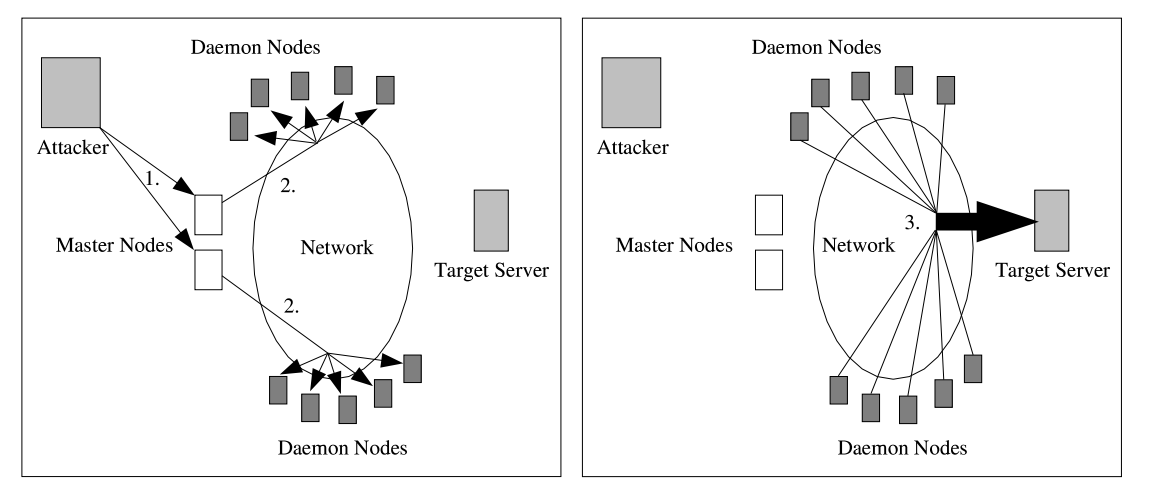
\includegraphics[width=1\textwidth]{Figures/ddos}
\decoRule
\caption[DDoS attack]{DDoS attack. \cite{hansman2005taxonomy}}
\label{fig:ddos}
\end{figure}

\subsection{Vulnerability scans}
\textbf{Network scans} are information gathering attacks. They do not cause any damage by themselves but usually serve the purpose to gather information about a system that could be used in further attacks. Network traffic sniffing or port scans are examples of network scans. \cite{IPFlow}

\subsection{Buffer overflows}
Buffer overflows are one of the most used methods of attacking a computer or network. They are
used to exploit flawed programming. They work by trying to overflow buffers within the program. When this happens the overflowed data will overflow into adjacent memory. This can cause data corruption or alter the execution of a program. There are stack-based and heap-based buffer overflows. Stack-based overflows try to overflow the program stack and heap-based overflows try to overflow dynamically created memory in a program. \cite{paulauskas2015computer}
 
\subsection{Brute-force attacks}
Brute-force attacks are a method that can be used to gain access to a target computer. This can be done by for example attempting all different kind of passwords. These attacks will eventually succeed but they can take a long time to execute. \cite{paulauskas2015computer}

\subsection{Physical attacks}
Physical attacks are attacks that try to physically damage computers. These attacks can be very basic, such as cutting a wire. However, they can also be energy attacks, such as  electro-magnetic pulses (EMP's) or high and low energy radio frequency (HERF and LERF) attacks. \cite{hansman2005taxonomy}

\subsection{Man in the Middle}
A man in the middle attack (MITM) is an attack where the attacker tries to secretly relay and possibly alter communication between two computers or networks as can be seen in Figure~\ref{fig:mitm}.  

\begin{figure}[H]
\centering
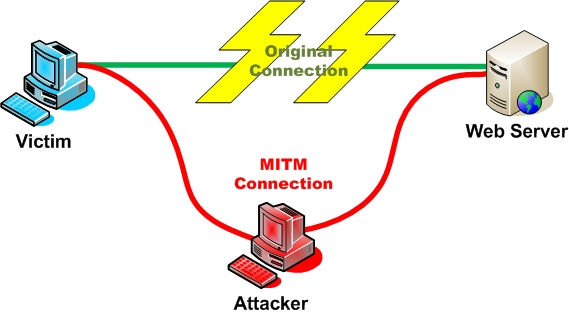
\includegraphics[width=1\textwidth]{Figures/main_the_middle}
\decoRule
\caption[Man in the middle attack]{Man in the middle attack. \cite{mitmExample}}
\label{fig:mitm}
\end{figure}

\section{Internal abnormal behaviour}
Internal abnormal behaviour can be called malware. There are several types of malware. There are four distinct categories of malware. There are \textbf{botnets}, \textbf{viruses}, \textbf{trojan horses} and \textbf{worms}. Malware are actual programs that infect a system to execute a specific task. The task of the malware defines which category the malware belongs in.

\subsection{Trojan horses}
\textbf{Trojan horses} are programs disguised as harmless applications but contain malicious code. They get their name from the battle of Troy. In stories it is said that the Greeks created a giant wooden horse and filled it with soldiers. The Trojans thought the horse was a gift of surrender. They brought the horse inside Troy. At night, the Greeks came out the horse, opened the gates of Troy and defeated Troy. This is also the way a Trojan horse works. Some of the capabilities of a Trojan horse include keystroke logging, program installation and file transfers. \cite{hansman2005taxonomy}

\subsection{Viruses}
\textbf{Viruses} are self-replicating programs that infect and spread through other programs. An infection means that they embed themselves within another program. When that program is run, the virus also activates and runs. \cite{hansman2005taxonomy}

\subsection{Worms}
\textbf{Worms} are programs that replicate themselves among a network.  They can spread extremely fast. Unlike viruses, they do not require infected files to spread. \cite{hansman2005taxonomy}

\subsection{Botnets}
\textbf{Botnets} is malware that causes infected computers to become "slaves" to the master. An infected computer is controlled externally by the bot-master without the knowledge of the owner of the infected computer. An example of this is shown in Figure~\ref{fig:botnet}. The bot-master can use the distributed network of "slave" computer to perform other malicious tasks, such as performing an DDOS attack. \cite{IPFlow}

\begin{figure}[H]
\centering
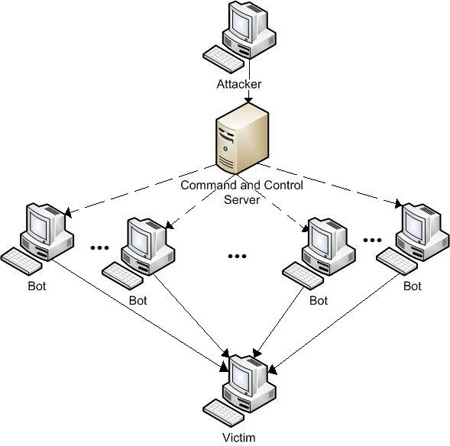
\includegraphics[width=0.6\textwidth]{Figures/botnet}
\decoRule
\caption[Botnet infection]{Botnet infection. \cite{botnetExample}}
\label{fig:botnet}
\end{figure}

\section{Detection}
An NIDS only monitors the network. As such not every attack can be detected by an NIDS. Only the attacks that actually use the network can be detected. Flow-based IDS have the additional constraint that they can only use flow data. This further limits the attacks that can be detected. The attacks that can generally be detected using a flow-based network intrusion detection systems are:
\begin{itemize}
\item DDOS
\item Vulnerability scans
\item Worms
\item Botnets
\end{itemize}
Other attacks either do not use network communication, or they are not visible within the header information of network traffic. In order to detect other attacks, including \textbf{Viruses}, \textbf{Trojan horses}, \textbf{Man in the Middle} and \textbf{Buffer overflows}, other detection systems such as HIDS or Packet-based NIDS should be used. \textbf{Physical attacks} are even more difficult to detect. \\\\
However there are some special circumstances in which other types of abnormal behaviour can be detected. When more information about a network and the abnormal behaviour is known, other types of abnormal behaviour can be detected. For example. when it is known that viruses are always distributed from the same source, it is possible to detect this distribution.This is  analogous for other attacks. \\\\
Other activities such as phoning home which a keystroke logging Trojan might do, could also be detected.  \textbf{Brute-force attacks} can also be detected since they might generate a lot of network traffic. However, unless the \textbf{Brute-force attack} is also a DDoS attack, the traffic mostly looks harmless from a flow-based approach. \cite{paulauskas2015computer}

\subsection{Distributed Denial of Service}
A distributed denial of service can be detected by the amount of data that is being received. However, there are many different types of DDoS attacks. There are ICMP floods, SYN floods, etc. These attacks can be described in terms of traffic patterns. A traffic pattern is expressed in a couple features. These features include the number of flows and packets, the packet size, and the total bandwidth used during the traffic. For example UDP flooding can be characterised by a traffic pattern which contains a lot of packets. These patterns can be searched for during the detection phase. \cite{kim2004flow}
\subsection{Network scans}
There are three categories of network scans.
\begin{itemize}
\item Horizontal scans: a single port is scanned across many different devices.
\item Vertical scan: several different ports are scanned on a single device
\item Block scan: a combination of both a vertical and a horizontal scan.
\end{itemize}
\noindent Scans can also be described using traffic patterns. They are characterised with a high number of flow and a low number of packets. These can again be used to detect whether a vertical or horizontal scan occurs. \cite{IPFlow} \cite{kim2004flow}

\subsection{Worms}
Worms exhibit different behaviour depending on their current state. There are two different states, a target discovery state and a transfer state. In the target discovery state, the worm explores the network to find vulnerabilities and a host to infect. During the transfer state, the worm actually transfers itself to the targeted host. The Sapphire/Slammer worm is an example of this type of behaviour. \cite{moore2003inside}\\
\\
Since transfering of the worm itself happens within the payload data, a flow-based NIDS cannot detect this state. The target discovery state can be detected. Worms use techniques similar to network scans in order to find vulnerable hosts. So similar detection techniques can be used to detect worms. \cite{abuadlla2014flow}

\subsection{Botnets}
Botnets usually consist out of a huge amount of infected slaves controlled by a central bot-master. Locating the individual infected slaves and isolating them is a difficult problem but is also insignificant due to the huge amount of remaining slaves. Detecting the bot-master and isolating that device is key to taking down a botnet. However indentifing botnet behaviour is a far more difficult problem than detection other types of malicious activities. \cite{zhu2008botnet} Malicious behaviour alone is not enough to detect botnets. \\
\\
Botnets often use IRC channels in order to communicate between slaves and the bot-master. These can be indentified using flows since they often use specific ports. It is possible to use a method that does not require specific port numbers. This requires flows including extra information such as the number of packets for which the PUSH flag is set.  


